\section*{Architekturmodellierung}
Ein funktionierendes System benötigt eine klare Architektur, die sicherstellt, dass Daten 
effizient verarbeitet, gespeichert und bereitgestellt werden.
Die Impfregistrierungsanwendung besteht aus mehreren technischen Komponenten, die 
zusammenarbeiten und einer Client-Server-Architektur folgen, bei der das
Frontend, Backend und die Datenbank klar voneinander getrennt sind.
Die Architekturmodellierung der Anwendung begann mit der Entwicklung eines Fachmodells, 
das die zentralen Entitäten und deren Beziehungen beschreibt. Dieses Modell diente als 
Grundlage für die funktionale Struktur der Anwendung und ermöglichte eine klare 
Definition der Geschäftslogik.

\begin{center}
  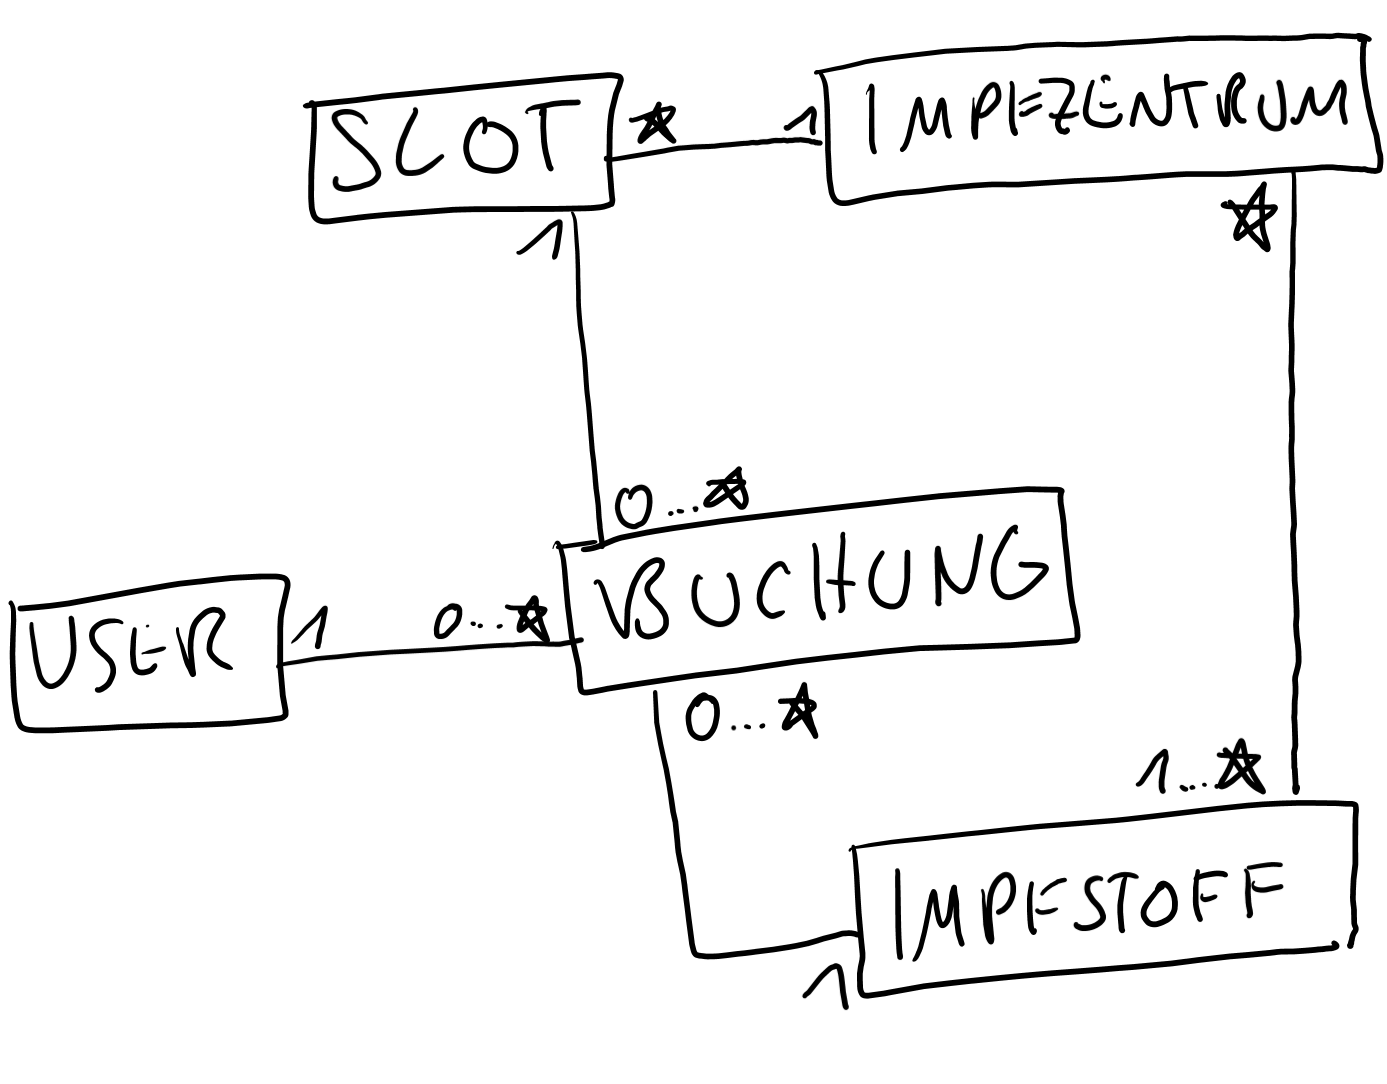
\includegraphics[width=0.95\linewidth, height=0.45\textheight, keepaspectratio]{src/abbildungen/fachmodell.PNG}
  \captionof{figure}{Fachmodell}
\end{center}

Basierend auf dem Fachmodell wurde anschließend ein relationales Datenmodell entwickelt, 
das die Speicherung und Verwaltung der Daten in der Datenbank strukturiert. 

\begin{center}
  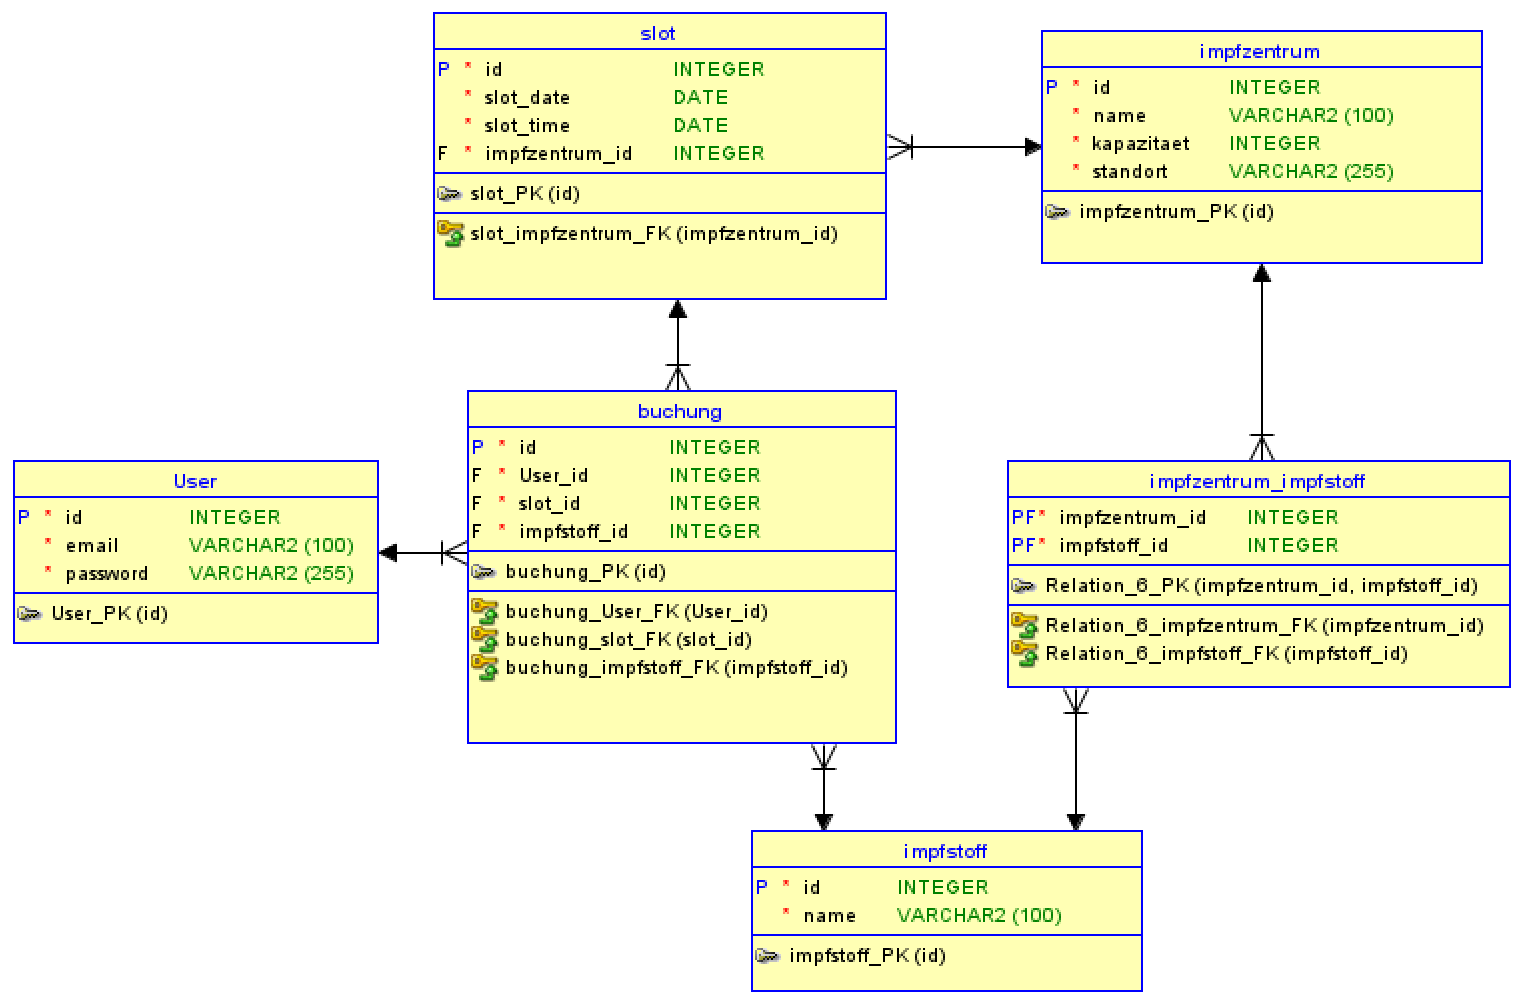
\includegraphics[width=0.95\linewidth, height=0.45\textheight, keepaspectratio]{src/abbildungen/relmodell.png}
  \captionof{figure}{Relationales Modell}
\end{center}
